\documentclass[12pt,a4paper]{article}

% ============================================================
% PACKAGES
% ============================================================
\usepackage[
    a4paper,
    top=1.55cm,
    bottom=1.35cm,
    left=1.75cm,
    right=1.75cm
]{geometry}

\usepackage[T1]{fontenc}
\usepackage{newtxtext}
\usepackage{graphicx}
\usepackage{xcolor}
\usepackage{array}
\usepackage{tabularx}
\usepackage{fancyhdr}
\usepackage{tikz}
\usepackage{eso-pic}
\usepackage{ragged2e}
\usepackage{enumitem}

% ============================================================
% COLORS
% ============================================================
\definecolor{GEUBlue}{RGB}{43,91,145}
\definecolor{GEUBannerBlue}{RGB}{0,102,148}
\definecolor{GEUYellow}{RGB}{255,201,38}
\definecolor{InstructionGrey}{RGB}{125,125,125}

% ============================================================
% GENERAL SETTINGS
% ============================================================
\setlength{\parindent}{0pt}
\setlength{\parskip}{0pt}
\renewcommand{\arraystretch}{1}

% ============================================================
% HEADER / FOOTER
% ============================================================
\pagestyle{fancy}
\fancyhf{}

\fancyhead[L]{%
    \fontsize{10.5}{12}\selectfont
    DSA Project Based Learning with C++
}

\fancyhead[R]{%
    \fontsize{10.5}{12}\selectfont
    PHASE-II PROJECT PROGRESS
}

\fancyfoot[R]{%
    \fontsize{10}{12}\selectfont
    Page \thepage
}

\renewcommand{\headrulewidth}{0pt}
\renewcommand{\footrulewidth}{0pt}

\setlength{\headheight}{20pt}
\setlength{\headsep}{0.65cm}
\setlength{\footskip}{0.65cm}

% ============================================================
% BOTTOM YELLOW LINE
% ============================================================
\AddToShipoutPictureBG{%
\begin{tikzpicture}[remember picture,overlay]
    \fill[GEUYellow]
    (current page.south west)
    rectangle
    ([yshift=0.14cm]current page.south east);
\end{tikzpicture}
}

% ============================================================
% CUSTOM COMMANDS
% ============================================================
\newcommand{\sectiontitle}[1]{%
    {\color{GEUBlue}
    \fontsize{18}{22}\selectfont #1}
}

\newcommand{\instruction}[1]{%
    {\color{InstructionGrey}
    \fontsize{10.5}{13}\selectfont #1}
}

% Auto-sizing answer box -- wraps tightly around whatever content is
% passed in, so long answers are never clipped by a fixed-height box.
\newcommand{\answerbox}[2][]{%
    \begin{tabularx}{\textwidth}{
        |>{\raggedright\arraybackslash}X|}
        \hline
        \parbox[t]{\dimexpr\linewidth-12pt\relax}{
            \vspace{5pt}
            \fontsize{11}{13}\selectfont #2
            \vspace{5pt}
        }\\
        \hline
    \end{tabularx}
}

% ============================================================
% DOCUMENT
% ============================================================
\begin{document}

% ============================================================
% PAGE 1
% ============================================================

\vspace*{0.10cm}


\includegraphics[width=8.0cm]{geulogo.png}

\vspace{0.70cm}

\noindent
\colorbox{GEUBannerBlue}{%
\parbox{\dimexpr\textwidth-2\fboxsep\relax}{
    \vspace{0.17cm}
    {\color{GEUYellow}
    \fontsize{16.5}{20}\selectfont
    \bfseries
    PROJECT AND TEAM INFORMATION}
    \vspace{0.17cm}
}}

\vspace{0.80cm}

% PROJECT TITLE
\sectiontitle{Project Title}

\vspace{0.05cm}

\vspace{0.40cm}

\answerbox{Vaultify -- A Secure Command-Line Password Manager in C++}

\vspace{0.80cm}

\noindent
\begin{tabularx}{\textwidth}{|>{\RaggedRight\arraybackslash}p{0.69\textwidth}|>{\RaggedRight\arraybackslash}X|}
\hline
\begin{minipage}[t]{\linewidth}
\vspace{1.5mm}
\textit{Team Id:}\\[-1mm]
\vspace{1.5mm}
\end{minipage}
&
\begin{minipage}[t]{\linewidth}
\vspace{1.5mm}
\textit{DSCPP-III-2026-T305}
\vspace{1.5mm}
\end{minipage}
\\
\hline
\begin{minipage}[t][3.9cm][t]{\linewidth}
\vspace{1.5mm}
\textbf{Team member 1 (Team Lead)}\\[-1mm]
\vspace{2mm}

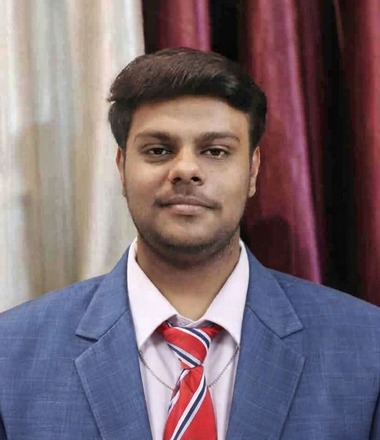
\includegraphics[width=1.9cm,height=2.2cm]{member1.jpg}
\end{minipage}
&
\begin{minipage}[t][3.9cm][t]{\linewidth}
\vspace{1.5mm}
\textit{Mishra, Ashraya}\\
\textit{Student ID: 2510010429}\\
\textit{Roll No.: 2027681}\\
\textit{Section : B}
\end{minipage}
\\
\hline
\begin{minipage}[t][3.9cm][t]{\linewidth}
\vspace{1.5mm}
\textbf{Team member 2}\\[-1mm]
\vspace{2mm}

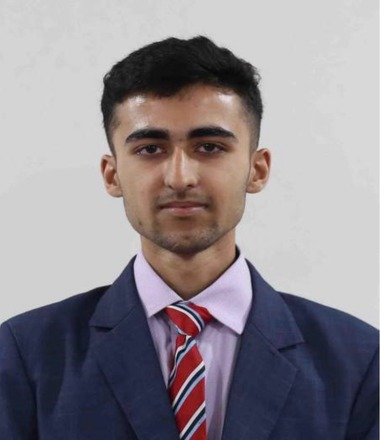
\includegraphics[width=1.9cm,height=2.2cm]{member2.jpg}
\end{minipage}
&
\begin{minipage}[t][3.9cm][t]{\linewidth}
\vspace{1.5mm}
\textit{Joshi, Udit}\\
\textit{Student ID: 2510370397}\\
\textit{Roll No.: 2028891}\\
\textit{Section : ML2}
\end{minipage}
\\
\hline
\begin{minipage}[t][3.9cm][t]{\linewidth}
\vspace{1.5mm}
\textbf{Team member 3}\\[-1mm]
\vspace{2mm}


\includegraphics[width=1.9cm,height=2.2cm]{member3.jpg}
\end{minipage}
&
\begin{minipage}[t][3.9cm][t]{\linewidth}
\vspace{1.5mm}
\textit{Singh, Yuvraj}\\
\textit{Student ID: 2510010591}\\
\textit{Roll No.: 2028915}\\
\textit{Section: ML3}
\end{minipage}
\\
\hline
\end{tabularx}

\newpage
% ============================================================
% PAGE 2
% ============================================================

\vspace*{0.15cm}

\noindent
\colorbox{GEUBannerBlue}{%
\parbox{\dimexpr\textwidth-2\fboxsep\relax}{
    \vspace{0.18cm}
    {\color{GEUYellow}
    \fontsize{17}{21}\selectfont
    \bfseries
    PHASE-II PROJECT PROGRESS DESCRIPTION}
    \vspace{0.18cm}
}}

\vspace{0.70cm}

% PROJECT ABSTRACT
\sectiontitle{Project Abstract}

\vspace{0.05cm}


\vspace{0.12cm}

\answerbox{Vaultify is a secure, offline, command-line password manager built in C++17 for a single user on a single machine. It addresses the widespread problem of password reuse and weak passwords by letting a user store strong, unique credentials for every account while remembering only one master password. The project is built from first principles rather than relying on existing libraries: credentials are stored in a manually implemented hash table (using separate chaining for collision resolution) that gives O(1) average lookup by site name; stored passwords are protected using a symmetric XOR cipher keyed on the master password; and the master password itself is never stored anywhere -- only a one-way hash of it is kept on disk and used purely for login verification. A dedicated FileHandler module persists the encrypted vault to a local flat file so data survives across sessions, and a menu-driven CLI ties every module together. The project deliberately applies core Data Structures concepts (hashing, collision resolution, stacks) and Object-Oriented Programming concepts (encapsulation, class design, file handling) taught in this course, rather than using built-in STL containers, so that the underlying mechanics are demonstrated rather than abstracted away.}

\vspace{0.70cm}

% UPDATED PROJECT APPROACH

\vspace{0.05cm}

\sectiontitle{Updated Project Approach}
\vspace{0.25cm}

\answerbox{The system is organized into six independent modules, each matching a single responsibility: \textbf{Entry} (the credential data class -- site, username, encrypted password, fully encapsulated), \textbf{Vault} (the hash table storage engine using separate chaining, with dynamic resizing once the load factor exceeds roughly 0.7), \textbf{Crypto} (the XOR symmetric cipher for encrypting/decrypting stored passwords, plus a custom djb2-style hash function used only to verify the master password at login -- never to decrypt data), \textbf{FileHandler} (serializes the vault to a pipe-delimited flat file and reconstructs it on startup), \textbf{RecentStack} (a LIFO stack tracking the last few retrieved sites), and \textbf{CLI} (the menu-driven interface that calls into the other modules but contains no business logic itself). This separation means the CLI could later be replaced with a GUI without touching any of the underlying logic. No external libraries or frameworks are used -- only the C++ standard library (\texttt{<string>}, \texttt{<vector>}, \texttt{<fstream>}, \texttt{<random>}) -- since the goal is to demonstrate the data structures and OOP concepts ourselves rather than depend on pre-built abstractions such as \texttt{std::unordered\_map}. The tool is single-process and local-only, so there is no network communication or client-server protocol involved; all "communication" is between in-process modules via well-defined class interfaces. Development uses Visual Studio Code with GCC/g++ (C++17), Git for version control, and the project compiles cleanly on both Windows (MinGW) and Linux with no platform-specific code paths.}

\newpage

% ============================================================
% PAGE 3
% ============================================================

\vspace*{0.20cm}

% TASKS COMPLETED
\sectiontitle{Tasks Completed (7 pts)}

\vspace{0.05cm}


\vspace{0.20cm}

\begin{tabularx}{\textwidth}{
|>{\raggedright\arraybackslash}X
|>{\raggedright\arraybackslash}X|
}
\hline
\textbf{Task Completed} &
\textbf{Team Member}\\
\hline

\parbox[t][1.6cm][t]{\linewidth}{\vspace{4pt}Vault module -- hash table with separate chaining, insert/retrieve/update/delete/list operations}
&
\parbox[t][1.6cm][t]{\linewidth}{\vspace{4pt}Ashraya Mishra}
\\
\hline

\parbox[t][1.4cm][t]{\linewidth}{\vspace{4pt}FileHandler module -- vault persistence (save/load) to a local encrypted flat file}
&
\parbox[t][1.4cm][t]{\linewidth}{\vspace{4pt}Ashraya Mishra}
\\
\hline

\parbox[t][1.4cm][t]{\linewidth}{\vspace{4pt}Entry class -- encapsulated credential data model}
&
\parbox[t][1.4cm][t]{\linewidth}{\vspace{4pt}Udit Joshi}
\\
\hline

\parbox[t][1.6cm][t]{\linewidth}{\vspace{4pt}Crypto module -- XOR cipher for password encryption/decryption and djb2-based master password hashing}
&
\parbox[t][1.6cm][t]{\linewidth}{\vspace{4pt}Udit Joshi}
\\
\hline

\parbox[t][1.6cm][t]{\linewidth}{\vspace{4pt}CLI module -- menu-driven interface, input validation, colored/formatted output}
&
\parbox[t][1.6cm][t]{\linewidth}{\vspace{4pt}Yuvraj Singh}
\\
\hline

\parbox[t][1.4cm][t]{\linewidth}{\vspace{4pt}RecentStack module and initial cross-platform (Windows/Linux) build testing}
&
\parbox[t][1.4cm][t]{\linewidth}{\vspace{4pt}Yuvraj Singh}
\\
\hline
\end{tabularx}

\vspace{0.65cm}

% CHALLENGES
\sectiontitle{Challenges/Roadblocks (7 pts)}

\vspace{0.05cm}


\vspace{0.18cm}

\answerbox{One early challenge was deciding how to resolve hash collisions in the Vault without relying on \texttt{std::unordered\_map} -- we evaluated open addressing against separate chaining and chose separate chaining, since it handles a higher load factor more gracefully and avoids the extra complexity of tombstone management needed when deleting entries under open addressing. A second challenge was a subtle design risk in Crypto: an early draft risked using the stored master-password hash itself as the decryption key, which would have meant anyone who stole the vault file could decrypt every entry without ever knowing the real password. We corrected this so the hash is used \emph{only} for login verification, while the actual decryption key is always the plain-text master password typed by the user in that session, never persisted anywhere. A third, ongoing challenge is keeping the hash table's performance genuinely O(1) as more entries are added -- we are implementing dynamic resizing (doubling the table and rehashing once load factor crosses roughly 0.7) to prevent long chains from degrading lookup speed. Finally, ensuring identical behavior on both Windows (MinGW) and Linux required care around file path handling and verifying that ANSI color codes render correctly across terminals; we are testing on both platforms in parallel rather than treating cross-platform support as an afterthought at the end.}

\vspace{0.65cm}

% TASKS PENDING
\sectiontitle{Tasks Pending}

\vspace{0.05cm}


\vspace{0.18cm}

\begin{tabularx}{\textwidth}{
|>{\raggedright\arraybackslash}X
|>{\raggedright\arraybackslash}X|
}
\hline

\textbf{Task Pending} &
\textbf{Team Member (to complete the task)}
\\
\hline

\parbox[t][1.4cm][t]{\linewidth}{\vspace{4pt}Dynamic hash table resizing when load factor exceeds threshold}
&
\parbox[t][1.4cm][t]{\linewidth}{\vspace{4pt}Ashraya Mishra}
\\
\hline

\parbox[t][1.4cm][t]{\linewidth}{\vspace{4pt}Random password generator and password-strength checker (stretch goals)}
&
\parbox[t][1.4cm][t]{\linewidth}{\vspace{4pt}Udit Joshi}
\\
\hline

\parbox[t][1.4cm][t]{\linewidth}{\vspace{4pt}Full regression testing across both platforms, final CLI polish, and README finalization}
&
\parbox[t][1.4cm][t]{\linewidth}{\vspace{4pt}Yuvraj Singh}
\\
\hline

\end{tabularx}

\newpage

% ============================================================
% PAGE 4
% ============================================================

\vspace*{0.30cm}

% PROJECT OUTCOME
\sectiontitle{Project Outcome/Deliverables}

\vspace{0.05cm}


\vspace{0.35cm}

\answerbox{The completed project will deliver: a fully functional, cross-platform C++ command-line password manager compiled and tested on both Windows and Linux; complete, well-commented source code implementing the Entry, Vault, Crypto, FileHandler, RecentStack, and CLI modules; a compiled executable ready for direct use; and a final report (with this progress document and the Phase-I proposal) documenting the design, security model, and stated limitations of the system. The core deliverable -- secure local storage and retrieval of credentials without ever storing the master password in plain text -- is already functioning end-to-end in the current build.}

\vspace{0.75cm}

% PROGRESS OVERVIEW
\sectiontitle{Progress Overview}

\vspace{0.05cm}


\vspace{0.25cm}

\answerbox{All five core goals from the Phase-I proposal are functionally in place: the hash table vault, XOR-based encryption/decryption, hash-based master password authentication, file persistence, and a working menu-driven CLI. This puts the project on schedule against the TA2 milestone defined in Phase-I. Ahead of schedule: the RecentStack feature (originally a stretch goal) and initial CLI output polish (colored, formatted output) are already implemented. Slightly behind schedule: dynamic hash table resizing is designed but not yet fully implemented, and the two remaining stretch goals (password generator, strength checker) have not been started. Both are scoped to be completed well before the TA3 final demonstration, and neither blocks the core, already-working functionality.}

\newpage

% ============================================================
% PAGE 5
% ============================================================

\vspace*{0.20cm}

% CODEBASE
\sectiontitle{Codebase Information }

\vspace{0.05cm}



\vspace{0.20cm}

\answerbox{Repository: \texttt{https://github.com/axhraya1121/password-manager} . Primary branch: \texttt{main}. Development follows a modular commit history aligned to the module ownership above -- key commits include the initial project scaffold (Entry, Vault, Crypto, FileHandler, CLI headers and build setup), the working Vault hash table with separate chaining, the Crypto module implementing the XOR cipher and djb2 master-password hashing with the hash-vs-encryption-key separation, the FileHandler persistence layer, and the CLI integration commit tying all modules together into a runnable end-to-end build. All members commit directly to \texttt{main} with regular small commits per completed sub-task, following the module boundaries defined in the Phase-I Project Approach.}

\vspace{0.65cm}

% TESTING
\sectiontitle{Testing and Validation Status }

\vspace{0.05cm}


\vspace{0.30cm}

\begin{tabularx}{\textwidth}{
|>{\raggedright\arraybackslash}p{0.34\textwidth}
|>{\raggedright\arraybackslash}p{0.31\textwidth}
|>{\raggedright\arraybackslash}X|
}
\hline

\textbf{Test Type} &
\textbf{Status (Pass/Fail)} &
\textbf{Notes}
\\
\hline

\parbox[t]{\linewidth}{\vspace{4pt}Vault insert/retrieve/update/delete}
&
\parbox[t]{\linewidth}{\vspace{4pt}Pass}
&
\parbox[t]{\linewidth}{\vspace{4pt}Verified O(1) average lookup behavior manually across varying entry counts}
\\
\hline

\parbox[t]{\linewidth}{\vspace{4pt}Encryption/decryption round-trip}
&
\parbox[t]{\linewidth}{\vspace{4pt}Pass}
&
\parbox[t]{\linewidth}{\vspace{4pt}Encrypted then decrypted passwords match original input exactly}
\\
\hline

\parbox[t]{\linewidth}{\vspace{4pt}Master password authentication}
&
\parbox[t]{\linewidth}{\vspace{4pt}Pass}
&
\parbox[t]{\linewidth}{\vspace{4pt}Correct password grants access; incorrect password rejected after 3 attempts}
\\
\hline

\parbox[t]{\linewidth}{\vspace{4pt}File persistence across sessions}
&
\parbox[t]{\linewidth}{\vspace{4pt}Pass}
&
\parbox[t]{\linewidth}{\vspace{4pt}Vault contents correctly reloaded after closing and relaunching the program}
\\
\hline

\parbox[t]{\linewidth}{\vspace{4pt}Cross-platform build}
&
\parbox[t]{\linewidth}{\vspace{4pt}Pass}
&
\parbox[t]{\linewidth}{\vspace{4pt}Compiled and run successfully on both Windows (MinGW) and Linux}
\\
\hline

\end{tabularx}

\vspace{0.65cm}

% DELIVERABLES PROGRESS
\sectiontitle{Deliverables Progress }

\vspace{0.05cm}


\vspace{0.25cm}

\answerbox{
\begin{itemize}[leftmargin=5mm, itemsep=2pt, topsep=2pt]
\item \textbf{Completed:} Entry class, Vault (hash table with separate chaining), Crypto (XOR cipher + master password hashing), FileHandler (persistence), RecentStack, and a working menu-driven CLI with colored output.
\item \textbf{In progress:} Dynamic hash table resizing; final cross-platform regression testing.
\item \textbf{Pending:} Random password generator and password-strength checker (stretch goals); final report and polished README.
\end{itemize}}

\end{document}